\section{UART}

%----------------------------------------------------------------------------------------
%	DEFINITION SUBESCTION
%----------------------------------------------------------------------------------------
\subsection{Definition}
A universal asynchronous receiver/transmitter , is a computer hardware device for asynchronous serial communication in which the data format and transmission speeds are configurable. The electric signaling levels and methods (such as differential signaling, etc.) are handled by a driver circuit external to the UART.\\

\centerline{
	\centering
	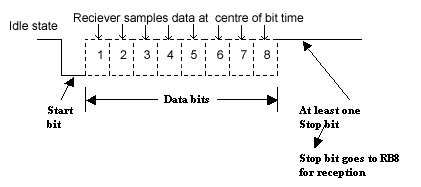
\includegraphics[width=1.0\textwidth]{overview/images/uart.png}
}
